\documentclass[a4paper,11pt]{article}

% Packages
\usepackage[utf8]{inputenc}
\usepackage[T1]{fontenc}
\usepackage[french]{babel}
\usepackage{fancyhdr}
\usepackage{geometry}
\usepackage{amsmath}
\usepackage{amssymb}
\usepackage{algorithm}
\usepackage{algpseudocode}
\usepackage{graphicx}

% Page layout
\geometry{a4paper, margin=2.5cm}

% Fix header height issue
\setlength{\headheight}{14pt}

% Header and footer setup
\pagestyle{fancy}
\fancyhf{} % Clear all header and footer fields

% Header
\fancyhead[R]{MIASHS - Outils financiers} % Right header

% Footer - with left, center, and right elements
\fancyfoot[L]{Boya | Seddouki } % Left footer
\fancyfoot[C]{Université de Clermont Auvergne} % Center footer
\fancyfoot[R]{\thepage} % Right footer

% Optional header/footer lines
\renewcommand{\headrulewidth}{0.4pt} % Header line (set to 0pt to remove)
\renewcommand{\footrulewidth}{0.4pt} % Footer line (set to 0pt to remove)

\begin{document}

    \begin{center}
        \Huge{MIASHS - Outils financiers}\\[0.5cm]
        \LARGE{Projet de mathématiques financières}\\[0.2cm]
        \Large{Erkin Tunc Boya | Rania Seddouki }\\
        \Large{Mars - Avril 2025}
    \end{center}

    \section{Introduction}

    \subsection{Contexte du projet}

    Dans le cadre de ce projet de mathématiques financières, nous nous intéressons à l’optimisation d’une stratégie d’investissement sur une période de temps donnée. Un investisseur dispose d’un capital initial qu’il peut placer de deux manières :
    \begin{itemize}
        \item à un taux d’intérêt de base constant appliqué à chaque période individuelle ;
        \item via des produits financiers spécifiques offrant des rendements plus intéressants, mais sur des intervalles plus longs.
    \end{itemize}

    Ces options sont limitées dans le temps et ne sont pas toujours disponibles simultanément. Cela soulève naturellement la question du meilleur enchaînement possible de placements pour maximiser le capital final.

    \subsection{Objectif et approche adoptée}

    L’objectif principal est de déterminer une politique d’investissement optimale permettant de maximiser le capital final à l’issue de la période d’étude.

    Pour résoudre ce problème, nous utilisons :
    \begin{itemize}
        \item une \textbf{modélisation mathématique} du problème sous forme d’un graphe orienté représentant les différentes possibilités de placements ;
        \item une \textbf{approche algorithmique} basée sur la programmation dynamique, évitant l’énumération exhaustive de toutes les possibilités, qui serait inefficace dès que l’horizon d’investissement devient important.
    \end{itemize}

    Dans la suite du rapport, nous allons présenter le modèle, illustrer son fonctionnement à travers un exemple concret, détailler les étapes algorithmiques et conclure par une analyse des résultats obtenus.


    

    \section{Modélisation mathématique}
    \subsection{Hypothèses et notations}

    L’horizon d’étude est une période discrète notée $T = [0, n]$, divisée en $n$ unités de temps. Un investisseur peut placer son capital de deux manières :
    \begin{itemize}
        \item \textbf{Placement de base} : À chaque période $[t, t+1]$, un taux d’intérêt fixe $\tau_0$ est appliqué. Il est disponible en continu sur toute la période $T$.
        \item \textbf{Placements spécifiques} : On dispose de $m$ opportunités de placement $P_k = (d_k, f_k, \tau_k)$ avec :
        \begin{itemize}
            \item $d_k$ : date de début du placement $k$ ;
            \item $f_k$ : date de fin du placement $k$ ;
            \item $\tau_k$ : taux d’intérêt applicable sur l’intervalle $[d_k, f_k]$.
        \end{itemize}
    \end{itemize}

    Chaque placement $P_k$ ne peut être utilisé qu’une seule fois et uniquement sur l’intervalle $[d_k, f_k]$.
    

    \subsection{Représentation par un graphe orienté}

    Pour modéliser ce problème, nous utilisons un graphe orienté noté $D = (V, A)$ :

    \begin{itemize}
        \item L’ensemble des \textbf{sommets} $V$ correspond aux dates $t \in \{0, 1, ..., n\}$.
        \item L’ensemble des \textbf{arcs} $A$ contient deux types de transitions :
        \begin{itemize}
            \item Les arcs de base $(t, t+1)$ avec un coefficient $c(t, t+1) = 1 + \tau_0$ ;
            \item Les arcs spécifiques $(d_k, f_k)$ correspondant aux produits d’investissement, avec $c(d_k, f_k) = 1 + \tau_k$.
        \end{itemize}
    \end{itemize}

    Chaque chemin dans ce graphe représente une stratégie d’investissement possible.


    \subsection{Chemins et stratégie de placement}

    Un \textbf{chemin} $P$ du sommet $0$ au sommet $n$ dans le graphe $D$ représente une séquence de décisions d’investissement. À chaque étape, le capital est multiplié par le coefficient de l’arc emprunté.

    On définit :
    \[
    C(P) = \prod_{a \in P} c(a)
    \]
    \indent comme le \textbf{coefficient multiplicatif total} associé à un chemin $P$.

    L’objectif est de déterminer le chemin $P^*$ tel que :
    \[
    C(P^*) = \max_{P \in \mathcal{P}(0, n)} C(P)
    \]

    où $\mathcal{P}(0, n)$ est l’ensemble des chemins allant de 0 à $n$ dans le graphe.

    Pour cela, on introduit une fonction de programmation dynamique :
    \[
    \text{Coef}(t) = \max_{P \in \mathcal{P}(0, t)} C(P)
    \]
    avec l’initialisation $\text{Coef}(0) = 1$. Cette fonction permet de calculer de manière séquentielle la valeur maximale atteignable à chaque date $t$.

    \subsection{Cardinalité des chemins dans le graphe}

    Le nombre de chemins possibles de 0 à $n$ dépend de la structure du graphe $D$.

    \paragraph{Cas général (avec seulement les arcs $(t, t+1)$)} 
    Si l’on ne considère que les placements de base (un seul arc $(t, t+1)$ entre deux dates consécutives), alors il n’existe qu’un seul chemin possible de 0 à $n$.

    \paragraph{Cas complet (tous les arcs $(t', t)$ possibles pour $t' < t$)} 
    Si le graphe contient tous les arcs $(t', t)$ avec $0 \leq t' < t \leq n$, alors le nombre total de chemins distincts de $0$ à $n$ est :
    \[
    |\mathcal{P}(0, n)| = 2^{n-1}
    \]

    \paragraph{Exemple : $n = 4$} 
    Dans ce cas, on a :
    \[
    |\mathcal{P}(0, 4)| = 2^{4-1} = 8
    \]
    Ce résultat s’explique par le fait que, à chaque étape intermédiaire $t \in \{1, 2, ..., n-1\}$, on a le choix : soit on continue avec un arc $(t, t+1)$, soit on saute directement à une date ultérieure (grâce à un arc $(t, t+k)$). Cela génère $2^{n-1}$ combinaisons possibles de décisions.

    \paragraph{Remarque} 
    Si le graphe est partiellement connecté (par exemple, uniquement certains arcs $(d_k, f_k)$ sont disponibles), alors le nombre de chemins doit être calculé au cas par cas en fonction des données fournies.


    \section{Étude d’un exemple concret}

    \subsection{Données du problème}

    Considérons une période d’étude de $n = 7$ unités de temps, avec un taux d’intérêt de base $\tau_0 = 0.009$ (0.9\% par période). L’investisseur dispose de cinq produits d’investissement spécifiques, caractérisés comme suit :

    \begin{center}
        \begin{tabular}{|c|c|c|c|}
        \hline
        Produit $k$ & Date début $d_k$ & Date fin $f_k$ & Taux $\tau_k$ (\%) \\
        \hline
        1 & 0 & 2 & 1.9 \\
        2 & 1 & 3 & 2.0 \\
        3 & 2 & 5 & 3.0 \\
        4 & 3 & 6 & 3.0 \\
        5 & 4 & 7 & 2.8 \\
        \hline
        \end{tabular}
    \end{center}

    \subsection{Construction du graphe}

    On construit un graphe orienté $D = (V, A)$ tel que :
    \begin{itemize}
        \item Les sommets $V = \{0, 1, ..., 7\}$ représentent les dates.
        \item Les arcs $(t, t+1)$ avec un taux $1 + \tau_0 = 1.009$ représentent les placements de base.
        \item Les arcs spécifiques $(d_k, f_k)$ avec coefficient $1 + \tau_k$ représentent les produits d’investissement disponibles.
    \end{itemize}

    Le graphe contient donc :
    \begin{itemize}
        \item Arcs de base : (0,1), (1,2), ..., (6,7)
        \item Arcs spécifiques : (0,2), (1,3), (2,5), (3,6), (4,7)
    \end{itemize}

    \begin{figure}[h!]
        \centering
        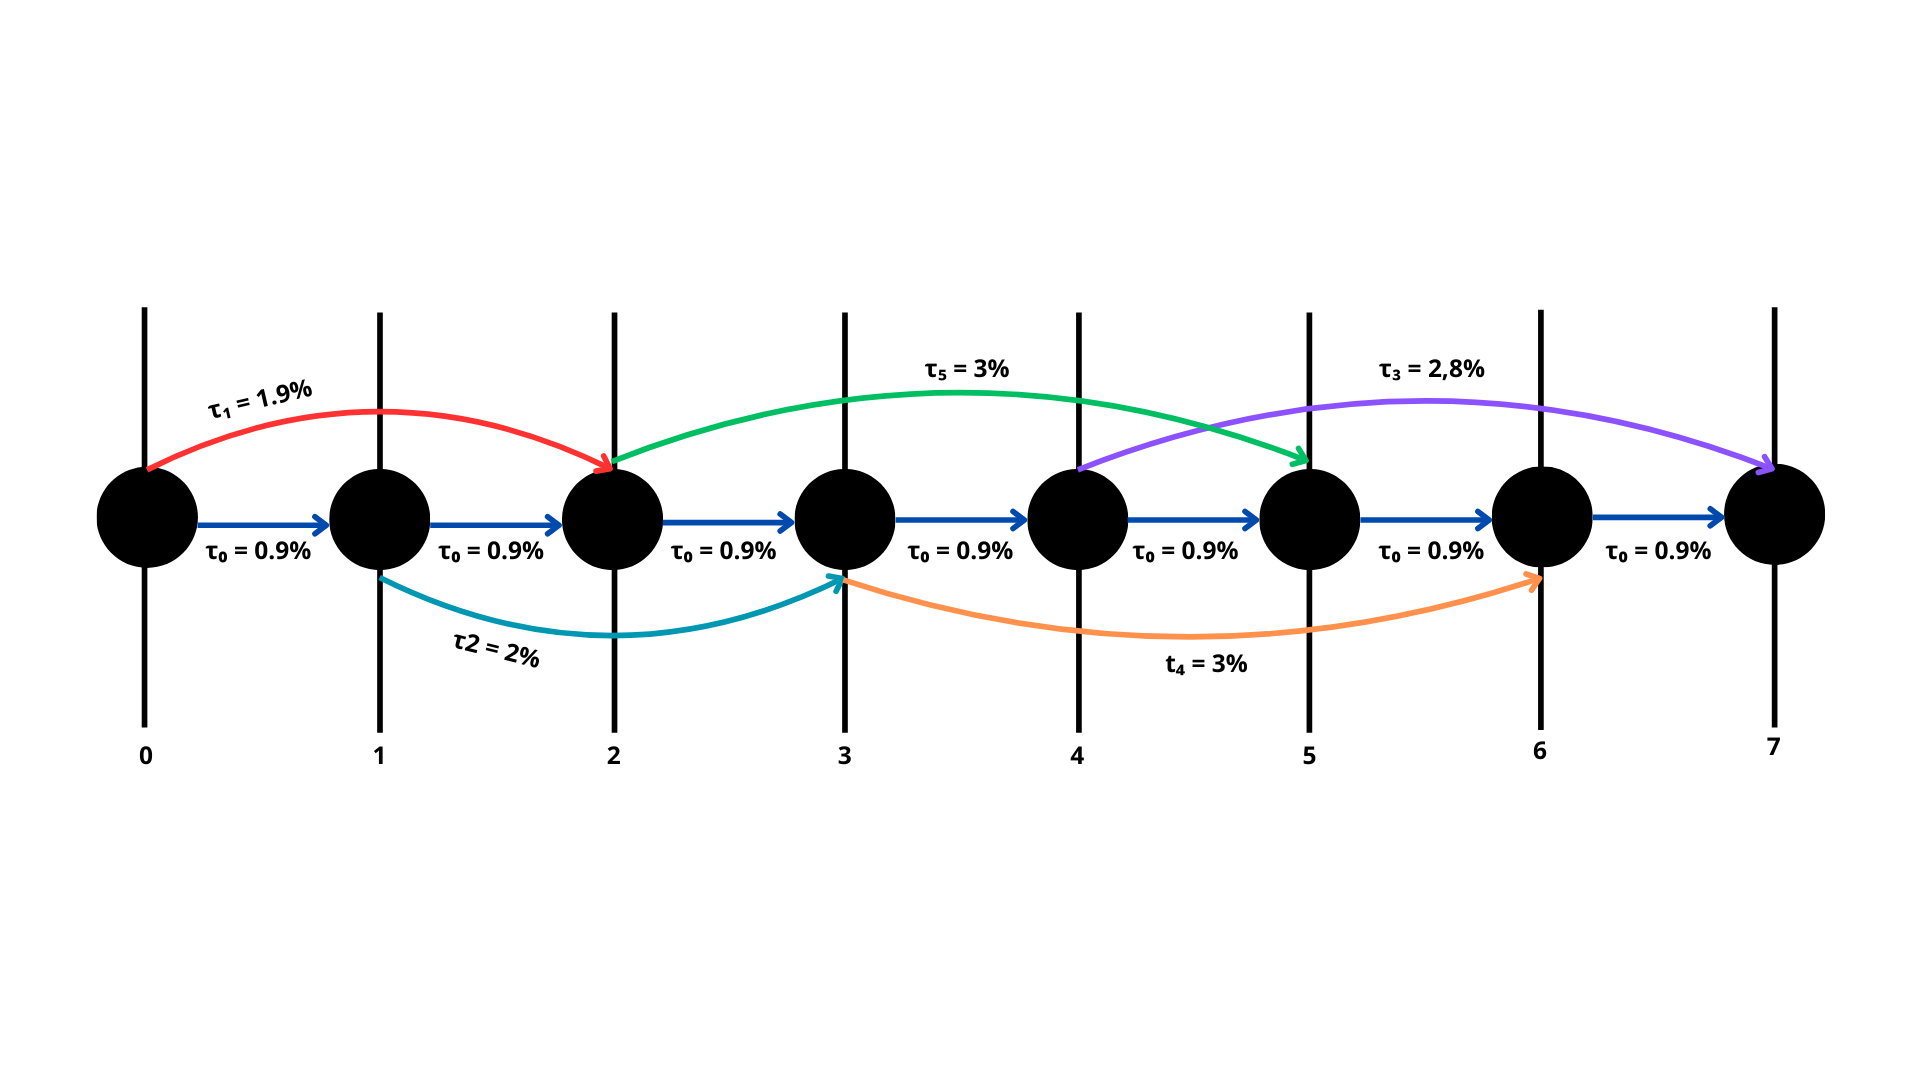
\includegraphics[width=0.85\textwidth]{images/graph_concret_exemple.png}
        \caption{Graphe orienté $D$ représentant les arcs $(t, t+1)$ et $(d_k, f_k)$ pour l'exemple avec $n = 7$.}
        \label{fig:graphe_exemple}
    \end{figure}

    \subsection{Évaluation de quelques chemins}

    Voici quelques chemins possibles de 0 à 7, et leur coefficient multiplicatif :

    \begin{itemize}
        \item Chemin 1 : $(0,1) \to (1,2) \to (2,3) \to (3,4) \to (4,5) \to (5,6) \to (6,7)$
    
        \hspace{0.5cm} $\Rightarrow C_1 = (1.009)^7 \approx 1.065$

        \item Chemin 2 : $(0,2) \to (2,3) \to (3,4) \to (4,5) \to (5,6) \to (6,7)$
    
        \hspace{0.5cm} $\Rightarrow C_2 = 1.019 \cdot (1.009)^5 \approx 1.066$

        \item Chemin 3 : $(0,2) \to (2,5) \to (5,6) \to (6,7)$
    
        \hspace{0.5cm} $\Rightarrow C_3 = 1.019 \cdot 1.03 \cdot (1.009)^2 \approx 1.069$

        \item Chemin 4 (optimal) : $(0,2) \to (2,5) \to (5,6) \to (6,7)$

        \hspace{0.5cm} Même que Chemin 3, mais confirmé comme optimal par comparaison.
    \end{itemize}

    \subsection{Cardinalité des chemins pour $n = 7$}
    Dans cet exemple, nous avons $n = 7$. Si l'on supposait que le graphe contient tous les arcs possibles $(t', t)$ avec $0 \leq t' < t \leq 7$, alors selon la formule théorique vue précédemment, le nombre total de chemins distincts de $0$ à $7$ serait :
    \[
    |\mathcal{P}(0, 7)| = 2^{7 - 1} = 64
    \]

    Cependant, dans notre cas particulier, seuls certains arcs $(d_k, f_k)$ sont disponibles, en plus des arcs de base $(t, t+1)$. Cela signifie que le graphe est partiellement connecté, et donc le nombre réel de chemins est inférieur à 64.

    Une énumération explicite ou une exploration du graphe permettrait de déterminer ce nombre avec précision. Cela justifie encore une fois l’intérêt d’une approche algorithmique dynamique plutôt que l’énumération brute, qui devient rapidement coûteuse.


    \subsection{Conclusion sur l’exemple}
    Le chemin $(0,2) \to (2,5) \to (5,6) \to (6,7)$ représente une stratégie optimale dans cet exemple. Il combine deux produits à taux élevé (1.9\%, 3.0\%) et termine avec des placements de base. Il permet de maximiser le coefficient multiplicatif total du capital, atteignant environ 1.069 — supérieur à toutes les stratégies fondées uniquement sur le taux de base.

    Cet exemple valide la nécessité d’utiliser une approche dynamique pour détecter efficacement la meilleure combinaison.



    \section{Recherche de la solution optimale}
    - Justification du besoin d’une approche dynamique
    - Formule de récurrence :
    \[
    \text{Coef}(t) = \max \left[ \text{Coef}(t-1) \cdot (1 + \tau_0), \max_{k \in N^{-}(t)} \left( \text{Coef}(d_k) \cdot (1 + \tau_k) \right) \right]
    \]
    - Propriété de D assurant l’existence de la solution

    \section{Implémentation algorithmique}
    \subsection{Lecture des données}
    - Fichier d’entrée, format des données

    \subsection{Fonction d’optimisation}
    - Calcul des Coef(t) de manière itérative

    \subsection{Procédure principale}
    - Algorithme général
    - Affichage des résultats

    \section{Résultats}
    - Meilleur chemin trouvé
    - Valeur finale maximale obtenue
    - Comparaison avec quelques chemins non-optimaux

    \section{Conclusion}
    - Résumé des apports
    - Limites de l’approche
    - Ouvertures possibles (gros n, taux variables...)
    
    \section*{Annexes}
    - Code source (Python)
    - Graphes dessinés à la main
    - Tableaux intermédiaires

\end{document}